\documentclass[11pt]{article}
\usepackage{fullpage}
\usepackage{amsfonts}
\usepackage{amsmath}
\usepackage{amsthm}
\usepackage{graphicx}
\usepackage{ulem}
\usepackage{framed}
\usepackage{url}

% Command for independent symbol
\def\ci{\perp}

% Command for not independent symbol
\def\notci{\not\perp}

% Packages for graphs and arrows
\usepackage{tikz}
\usetikzlibrary{arrows, calc, positioning, fit}

% Package for forcing figure placement
\usepackage{float}

\begin{document}

\title{CS 5526 -- Virginia Tech\\
	Homework 1}
\author{Brennon Bortz \\ (PID: brennon, Campus: Blacksburg)}
\date{11 March 2015}
\maketitle

Code for this assignment is available at \url{https://github.com/brennon/cs5526-hw1}. Python notebooks for Question 5 are available at \url{http://goo.gl/SeQn1b} (Na\"ive Bayes Classifier) and \url{http://goo.gl/BZdYD1} (Tree-Augmented Na\"ive Bayes Classifier).

\section*{Written Problems}

\begin{enumerate}

\item (10 points) Give an example of a decomposition of a joint probability distribution that cannot be captured by a Bayesian network.

\textbf{Solution:} The graph structure of Figure \ref{fig:impossible} with the following as the only independencies cannot be represented by a Bayesian network: $(A \ci D | B,C)$ and $(B \ci C | A,D)$.

\begin{figure}[H]
\centering
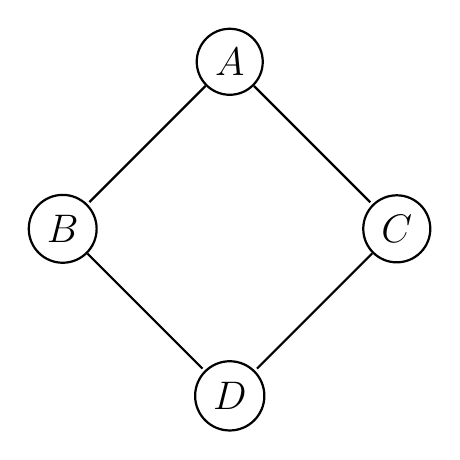
\begin{tikzpicture}[-,>=stealth',shorten >=1pt,auto,node distance=3cm,
                    thick,main node/.style={circle,draw,font=\sffamily\Large\bfseries}]

  \node[main node] (A) {$A$};
  \node[main node] (B) [below left of=A] {$B$};
  \node[main node] (C) [below right of=A] {$C$};
  \node[main node] (D) [below right of=B] {$D$};

  \path[every node/.style={font=\sffamily\small}]
    (A) edge node [] {} (B)
    (A) edge node [] {} (C)
    (C) edge node [] {} (D)
    (B) edge node [] {} (D);
    
\end{tikzpicture}
\caption{Impossible Bayesian network.}
\label{fig:impossible}
\end{figure}

\item (10 points) How many possible Bayesian networks are there involving three random variables? Group these networks into equivalence classes where each class contains networks that encode the same (conditional) independence assumptions.

\textbf{Solution:} There are 25 possible Bayesian networks involving three variables, comprising 8 different equivalence classes. Each row in Table \ref{fig:possible} shows one of these possible networks. An arrow in one of the first three columns indicates the direction of the edge connecting the nodes given in the header row. A check in one of the last three columns indicates the conditional independency in the header row holds given the edges indicated in the first three columns. Where two rows share the same pattern of check in the last three columns, they are members of the same equivalence class.

\begin{table}[h]
\centering
\begin{tabular}{c|c|c||c|c|c}
X-Y & Y-Z  & X-Z & $X \ci Y | Z$ & $X \ci Z | Y$ & $Y \ci Z | X$ \\
\hline
 &  &  & $\checkmark$ & $\checkmark$ & $\checkmark$\\
 & $\leftarrow$ &  & $\checkmark$ & $\checkmark$ & \\
 & $\rightarrow$ &  & $\checkmark$ & $\checkmark$ & \\
 &  & $\leftarrow$ & $\checkmark$ &  & $\checkmark$\\
 &  & $\rightarrow$ & $\checkmark$ &  & $\checkmark$\\
 & $\leftarrow$ & $\rightarrow$ & $\checkmark$ &  & \\
 & $\rightarrow$ & $\leftarrow$ & $\checkmark$ &  & \\
$\leftarrow$ &  &  &  & $\checkmark$ & $\checkmark$\\
$\rightarrow$ &  &  &  & $\checkmark$ & $\checkmark$\\
 & $\leftarrow$ & $\leftarrow$ &  & $\checkmark$ & \\
$\leftarrow$ & $\leftarrow$ &  &  & $\checkmark$ & \\
$\leftarrow$ & $\rightarrow$ &  &  & $\checkmark$ & \\
$\rightarrow$ & $\rightarrow$ &  &  & $\checkmark$ & \\
$\leftarrow$ &  & $\rightarrow$ &  &  & $\checkmark$\\
$\rightarrow$ &  & $\leftarrow$ &  &  & $\checkmark$\\
$\rightarrow$ &  & $\rightarrow$ &  &  & $\checkmark$\\
 & $\rightarrow$ & $\rightarrow$ &  &  & \\
$\leftarrow$ &  & $\leftarrow$ &  &  & \\
$\leftarrow$ & $\leftarrow$ & $\leftarrow$ &  &  & \\
$\leftarrow$ & $\rightarrow$ & $\leftarrow$ &  &  & \\
$\leftarrow$ & $\rightarrow$ & $\rightarrow$ &  &  & \\
$\rightarrow$ & $\leftarrow$ &  &  &  & \\
$\rightarrow$ & $\leftarrow$ & $\leftarrow$ &  &  & \\
$\rightarrow$ & $\leftarrow$ & $\rightarrow$ &  &  & \\
$\rightarrow$ & $\rightarrow$ & $\rightarrow$ &  &  & 
\end{tabular}
\caption{Possible Bayesian networks in three variables.}
\label{fig:possible}
\end{table}

\item (10 points) In the attached diagram (next page) assume that B and M are instantiated (i.e., evidence is introduced for these variables). List all the random variables that A is conditionally independent of.

\textbf{Solution:} $A$ is only independent of $G$ given $B$ and $M$.

\item (20 points) From Project Gutenberg, download the two files The Adventures of Sherlock Holmes by Arthur Conan Doyle (http://www.gutenberg.org/cache/epub/1661/pg1661.txt) and The Complete Works of Jane Austen (http://www.gutenberg.org/cache/epub/31100/pg31100.txt). Design a Markov sequence model that learns from each of these files (separately) and learns to write like Doyle or write like Austen. Note that your model need not be a HMM, just a probabilistic sequence model that predicts what the next word should be based on the current word (or current + past words, or some longer history). If you are adventurous, you can also explore the so-called skip gram models. How many bits of history would you need to use to create a realistic model, for each author? What are the disadvantages of using more history to form your model? For full credit, give an explanation of the experiments you tried and one example of a pseudo-Doyle document and one example of a pseudo-Austen document (1 page max each).

\textbf{Solution:} In my opinion, using 3-grams creates the most realistic output text for both authors. If the n-grams are shorter, the text makes little sense. If the n-grams are longer, the frequencies of any given n-gram are much lower. This causes the model to copy large sections of text wholesale from the original text, which is not the intended result. In addition to this, using less history is much faster and requires far less memory. I attempted both models with 1-, 2-, 3-, and 4-grams.

\textit{Doyle sample:}

As to what you tell me of poor Mary, it goes to my very heart. Not even your skill can inform me where she is now." "I think that we may gain that by means of the law; but we have our web to weave, while theirs is already woven. The first consideration is to remove the pressing danger which threatens you. The second is to clear up the mystery and to punish the guilty parties." "I thank you," said the young man, rising and pulling on his overcoat. "You have given me fresh life and hope. I shall certainly do as you advise." "Do not lose an instant. And, above all, take care of yourself in the meanwhile, for I do not think that any burglar could have done. "And now I have a very strange experience to tell you. I can assure you that it has not detracted in the tiniest iota from your appearance. We shall now see how the electric-blue dress will become you. You will find it here, and may read it for yourself." He picked out from his bundle a copy of the local Herefordshire paper, and having turned down the sheet he pointed out the paragraph in which the unfortunate bridegroom moves. Fresh scandals have eclipsed it, and their more piquant details have drawn the gossips away from this four-year-old drama. As I have reason to know that there are widespread rumours as to the death of Dr. Grimesby Roylott which tend to make the matter even more terrible than the truth. It was early in April in the year '83 that I woke one morning to find Sherlock Holmes standing, fully dressed, by the side of my bed. He was a late riser, as a rule, and as the clock makes it a few minutes after I found, rather, I confess, to my relief, that instead of being identified as Mr. Neville St. Clair, with the exception of his coat. His boots, his socks, his hat, and his right hand and sleeve were observed to be stained with fresh blood. On following him they found the dead body stretched out upon the grass beside the pool. The head had been beaten in by repeated blows of some heavy and blunt weapon. The injuries were such as might very well have been inflicted by the butt-end of his son's gun, which was found lying on the grass within a few paces of the body. Under these circumstances the young man was instantly arrested, and a verdict of 'wilful murder' having been returned at the inquest on Tuesday, he was on Wednesday brought before the magistrates at Ross, who have referred the case to the next Assizes. Those are the main facts of the case as they came out before the coroner and the police-court." "I could hardly imagine a more damning case," I remarked. "If ever circumstantial evidence pointed to a criminal it does so here." "Circumstantial evidence is a very tricky thing,"...

\textit{Austen sample:}

\item (50 points) Consider the Mushroom dataset from the UCI machine learning repository. Develop a Naive Bayes classifier and a tree-augmented Naive Bayes classifier to classify this dataset. Separate the data into training and test (describe what percentages you used) and report quantitative results after k-fold cross-validation. (Choose k suitably.) Interpret your experimental results and analyze if the tree-augmented classifier provides an improvement. You are welcome to code up the classifiers from scratch or use some ready made software for parts of the assignment, but must document what you did (e.g., software, languages used) and provide a public URL where any code/scripts written are made available.

Finally, I should note that I used the \verb|Counter| class available from the UC Berkeley CS 188 course source code.\footnote{\url{https://s3-us-west-2.amazonaws.com/cs188websitecontent/projects/release/search/v1/001/docs/util.html}}

\textbf{Solution:} For each classifier (see above for links to source and iPython notebooks), I used 10-fold cross validation to acheive the following results:

\begin{table}[h]
\centering
\begin{tabular}{c|c}
Network Type & Accuracy \\
\hline
Na\"ive Bayes Classifier & 99.4334\% \\
Tree-Augmented Na\"ive Bayes Classifier & 99.9507\% \\
\end{tabular}
\caption{NBC and TA-NBC accuracies on UCI mushroom dataset.}
\label{fig:possible}
\end{table}

While the TA-NBC did provide an improvement over the NBC, it was slight. Furthermore, the additional effort involved in hand-coding the TA-NBC was hardly worth the effort given this minimal increase in accuracy.

To implement these networks, I used the \verb|libpgm| Python library\footnote{\url{http://pythonhosted.org/libpgm/}}. For the TA-NBC in particular, however, much of the implementation was created by myself, as the library does not support TA-NBCs directly.

\end{enumerate}

\end{document}


